\newif\ifshowsolutions
\showsolutionstrue
\input{./preamble}



%%%%%%%%%%%%%%%%%%%%%%%%%%%%%%
% HEADER
%%%%%%%%%%%%%%%%%%%%%%%%%%%%%%

\chead{
  {\vbox{
      \vspace{2mm}
      \large
      Machine Learning \& Data Mining \hfill
      Caltech CS/CNS/EE 155 \hfill \\[1pt]
      Set 4\hfill
      February $7^\text{th}$, 2023 \\
    }
  }
}

\begin{document}
\pagestyle{fancy}



%%%%%%%%%%%%%%%%%%%%%%%%%%%%%%
% POLICIES
%%%%%%%%%%%%%%%%%%%%%%%%%%%%%%

\section*{Policies}
\begin{itemize}
  \item Due 9 PM, February $7^\text{th}$, via Gradescope.
  \item You are free to collaborate on all of the problems, subject to the collaboration policy stated in the syllabus.
  \item You should submit all code used in the homework. We ask that you use Python 3.6+ and PyTorch version 1.4.0 for your code, and that you comment your code such that the TAs can follow along and run it without any issues.
    \item This set requires the installation of PyTorch. There will be a recitation and office hour dedicated to helping you install these packages if you have problems.
\end{itemize}

\section*{Submission Instructions}
\begin{itemize}
   \item Please submit your report as a single .pdf file to Gradescope (entry code 9YJGEX), under "Problem Set 4". \textbf{In the report, include any images generated by your code along with your answers to the questions.} For instructions specifically pertaining to the Gradescope submission process, see \url{https://www.gradescope.com/get_started#student-submission}.
   
   \item Since we are only using Gradescope this year, we ask that you upload both your code and solution pdf together as a single pdf and mark each page with the problem number. There are various free online tools to combine pdfs. To download your code as a pdf from Jupyter notebook, you can navigate to File -$>$ Download as -$>$ "PDF via Latex" or alternatively download the Latex file and compile it yourself.
\end{itemize}

\section*{TA Office Hours}
\begin{itemize}
    \item \textbf{Julio Arroyo}
        \begin{itemize}
            \item Sunday, 2/5: 3:00 pm - 4:00 pm
            \item Monday, 2/6: 8:00 pm - 9:00 pm
        \end{itemize}
    \item \textbf{Sreemanti Dey}
        \begin{itemize}
            \item Friday, 2/3: 7:00 pm - 8:00 pm
            \item Monday, 2/6: 7:00 pm - 8:00 pm
        \end{itemize}
\end{itemize}

%%%%%%%%%%%%%%%%%%%%%%%%%%%%%%
% PROBLEM 1
%%%%%%%%%%%%%%%%%%%%%%%%%%%%%%

\newpage
\section{Deep Learning Principles [35 Points]}
\materials{lectures on deep learning}

 For problems A and B, we'll be utilizing the \href{http://playground.tensorflow.org/}{Tensorflow Playground} to visualize/fit a neural network.

\begin{problem}[5]
  Backpropagation and Weight Initialization Part 1
\end{problem}

Fit the neural network at \href{http://playground.tensorflow.org/#activation=relu&batchSize=10&dataset=circle&regDataset=reg-plane&learningRate=0.03&regularizationRate=0&noise=0&networkShape=4,2&seed=0.65409&showTestData=false&discretize=false&percTrainData=50&x=true&y=true&xTimesY=false&xSquared=false&ySquared=false&cosX=false&sinX=false&cosY=false&sinY=false&collectStats=false&problem=classification&initZero=false&hideText=false}{this link} for about 250 iterations, and then do the same for the neural network at  \href{http://playground.tensorflow.org//\#activation=relu&batchSize=10&dataset=circle&regDataset=reg-plane&learningRate=0.03&regularizationRate=0&noise=0&networkShape=4,2&seed=0.6&showTestData=false&discretize=false&percTrainData=50&x=true&y=true&xTimesY=false&xSquared=false&ySquared=false&cosX=false&sinX=false&cosY=false&sinY=false&collectStats=false&problem=classification&initZero=true&hideText=false}{this link}.  Both networks have the same architecture and use ReLU activations.  The only difference between the two is how the layer weights were initialized -- you can examine the layer weights by hovering over the edges between neurons.

Give a mathematical justification, based on what you know about the backpropagation algorithm and the ReLU function, for the difference in the performance of the two networks.

\begin{subsolution}

\end{subsolution}

\begin{problem}[5]
  Backpropagation and Weight Initialization Part 2
\end{problem}
Reset the two demos from part i (there is a reset button to the left of the ``Run'' button), change the activation functions of the neurons to sigmoid instead of ReLU, and train each of them for 4000 iterations.

Explain the differences in the models learned, and the speed at which they were learned, from those of part i in terms of the backpropagation algorithm and the sigmoid function.



\begin{subsolution}

\end{subsolution}



\problem \textbf{[10 Points]}

When training any model using SGD, it's important to shuffle your data to avoid correlated samples. To illustrate one reason why this is particularly important for ReLU networks (i.e. it has ReLU activation functions between its hidden layers, but its output layer is still softmax/tanh/linear), consider a dataset of 1000 points, 500 of which have positive (+1) labels, and 500 of which have negative (-1) labels. What happens if we train a fully-connected network with ReLU activations using SGD, looping through all the negative examples before any of the positive examples? Do not assume that the derivative of ReLU at 0 is implemented as 0. \textit{Hint: this is called the ``dying ReLU'' problem, although it is possible with other activation functions.}

\textit{}

\begin{solution}

\end{solution}



\problem Approximating Functions Part 1 \textbf{[7 Points]}

Draw or describe a fully-connected network with ReLU units that implements the OR function on two 0/1-valued inputs,  $x_1$ and $x_2$.  Your networks should contain the minimum number of hidden units possible.  The OR function $\text{OR}(x_1, x_2)$ is defined as:
\begin{gather*}
\text{OR}(1, 0) \geq 1 \\
\text{OR}(0, 1) \geq 1 \\
\text{OR}(1, 1) \geq 1 \\
\text{OR}(0, 0) = 0
\end{gather*}

Your network need only produce the correct output when $x_1 \in \{0, 1\}$ and $x_2 \in \{0, 1\}$ (as described in the examples above).

\begin{subsolution}

\end{subsolution}

\problem Approximating Functions Part 2 \textbf{[8 Points]}

What is the minimum number of fully-connected layers (with ReLU units) needed to implement an XOR of two 0/1-valued inputs $x_1, x_2$? Recall that the XOR function is defined as:
\begin{gather*}
\text{XOR}(1, 0) \geq 1 \\
\text{XOR}(0, 1) \geq 1 \\
\text{XOR}(0, 0) = \text{XOR}(1, 1) = 0
\end{gather*}

For the purposes of this problem, we say that a network $f$ computes the XOR function if $f(x_1, x_2) = \text{XOR}(x_1, x_2)$ when $x_1 \in \{0, 1\}$ and $x_2 \in \{0, 1\}$ (as described in the examples above).

Explain why a network with fewer layers than the number you specified cannot compute XOR.


\begin{subsolution}

\end{subsolution}


% problem 3
\newpage
\section{Inside a Neural Network  [17 Points]}

\textit{Relevant Materials: Lectures on Deep Learning}

Although this is no longer the peak of the pandemic, coronavirus datasets are still very salient due to the number of people in the US that are still being affected by the disease. In this problem, you will investigate the workings of a simple neural network by designing linear neural nets to classify coronavirus cases.

\medskip

\problem \textbf{Installation} \textbf{[2 Points]}

Before any modeling can begin, PyTorch must be installed. PyTorch is an automatic differentiation framework that is widely used in machine learning research.  We will also need the \textbf{torchvision} package later on, which will make downloading the MNIST dataset much easier. 

To install both packages, follow the steps on \\
\url{https://pytorch.org/get-started/locally/#start-locally}. Select the 'Stable' build and your system information. We highly recommend using Python 3.6+. CUDA is not required for this class, but it is necessary if you want to do GPU-accelerated deep learning in the future.

Once you have finished installing, write down the version numbers for both \textbf{torch} and \textbf{torchvision} that you have installed.

\begin{solution}

\end{solution}

\problem \textbf{The Data} \textbf{[5 Points]}

Load and preprocess the tabular dataset, "COVID-19\_Case\_Surveillance\_Public\_Use\_Data\_Subset.csv." This is a small subset of the CDC's Covid-19 Case Surveillance data (\url{https://data.cdc.gov/Case-Surveillance/COVID-19-Case-Surveillance-Public-Use-Data/vbim-akqf}). Limit the number of input variables in your final dataset to be between 7 and 12, and use the "death\_yn" column as the dependent variable. You might find various features in the pandas package useful here.

Explain your preprocessing decisions.

\begin{solution}

\end{solution}


\problem \textbf{Linear Neural Network} \textbf{[5 Points]}

Now, use PyTorch's "Sequential" class to make a neural network with one linear layer of size 5 and a binary output layer (with softmax, since this is a classification task). Do not use any activation function in your linear layer. Choose an appropriate optimizer, learning rate, and loss function (either Adam or RMSProp will probably work best as an optimizer). Use these to train and test your model on your dataset--look at the problem 3 sample code to see how to train and test.

Finally, visualize the weight vectors in your model with a heatmap.

Make sure to show training losses and test accuracy clearly in your notebook.

\begin{solution}

\end{solution}


\problem \textbf{2-Layer Linear Neural Network} \textbf{[5 Points]}

Finally, create and train a 2-layer linear neural network and assess its performance on your dataset. It is expected that the 1-layer and 2-layer models have very similar losses--why is this the case?

\begin{solution}

\end{solution}





% problem 3
\newpage
\section{Depth vs Width on the MNIST Dataset  [23 Points]}

\textit{Relevant Materials: Lectures on Deep Learning}

MNIST is a classic dataset in computer vision. It consists of images of handwritten digits (0 - 9) and the correct digit classification. In this problem you will implement a deep network using PyTorch to classify MNIST digits. Specifically, you will explore what it really means for a network to be "deep", and how depth vs. width impacts the classification accuracy of a model. You will be allowed at most $N$ hidden units, and will be expected to design and implement a deep network that meets some performance baseline on the MNIST dataset.

\medskip

\problem \textbf{The Data} \textbf{[3 Points]}

Load the MNIST dataset using torchvision; see the problem 3 sample code for how.

Image inputs in PyTorch are generally 3D tensors with the shape (no. of channels, height, width). Examine the input data. What are the height and width of the images? What do the values in each array index represent?  How many images are in the training set? How many are in the testing set? You can use the \textbf{imshow} function in matplotlib if you'd like to see the actual pictures (see the sample code).

\begin{subsolution}

\end{subsolution}

\subsection{Model submission instructions: }
For each problem 3C-3E and 4G \underline{there should be a separate notebook.} In your notebook, include the code you used to train your model and make sure your results are visible.

 \problem \textbf{Modeling Part 1} \textbf{[8 Points]}

 Using PyTorch's "Sequential" model class, build a deep network to classify the handwritten digits. You may \textbf{only} use the following layers:

 \begin{itemize}
  \item \textbf{Linear:} A fully-connected layer
  \item \textbf{ReLU (activation):} Sets negative inputs to 0
  \item \textbf{Softmax (activation):} Rescales input so that it can be interpreted as a (discrete) probability distribution.
  \item \textbf{Dropout:} Takes some probability and at every iteration sets weights to zero at random with that probability (effectively regularization)
\end{itemize}

A sample network with 20 hidden units is in the sample code file. (Note: activations, Dropout, and your last Linear layer do not count toward your hidden unit count, because the final layer is ``observed'' and not \emph{hidden}.)

Use categorical cross entropy as your loss function. There are also a number of optimizers  you can use (an optimizer is just a fancier version of SGD), and feel free to play around with them, but RMSprop and Adam are the most popular and will probably work best. You also should find the batch size and number of epochs that give you the best results (default is batch size = 32, epochs=10).

Look at the sample code to see how to train your model. PyTorch should make it very easy to tinker with your network architecture.

\textbf{Your task}. Using at most 100 hidden units, build a network using only the allowed layers that achieves test accuracy of at least 0.975.

\textbf{Imporant note on stochasticity: } For problems 3C-3E and 4G, you might notice that your model's accuracy fluctuates every time you train it. This is caused by weight initialization, shuffled mini-batching for SGD, dropout probabilities, etc. You may want to consider controlling the effects of randomness by \href{https://pytorch.org/docs/stable/generated/torch.manual_seed.html}{manually setting the seed}. In any case, when we say "achieve test accuracy of at least $x$", we mean that your model should achieve the stated accuracy more than half the times you train it.

\textit{Hint}: for best results on this problem and the two following problems, normalize the input vectors by dividing the values by 255 (as the pixel values range from 0 to 255).

\begin{solution}

\end{solution}


 \problem \textbf{Modeling Part 2} \textbf{[6 Points]}

 Repeat problem C, except that now you may use 200 hidden units and must build a model with at least 2 hidden layers that achieves test accuracy of at least 0.98.

 \begin{solution}

\end{solution}

  \problem \textbf{Modeling Part 3} \textbf{[6 Points]}

 Repeat problem C, except that now you may use 1000 hidden units and must build a model with at least 3 hidden layers that achieves test accuracy of at least 0.983.

  \begin{solution}

\end{solution}

 \newpage
 % problem 4
 \section{Convolutional Neural Networks  [40 Points]}
 \textit{Relevant Materials: Lecture on CNNs}

 \problem Zero Padding \textbf{[5 Points]}

 Consider a convolutional network in which we perform a convolution over each $8 \times 8$ patch of a $20 \times 20$ input image. It is common to zero-pad input images to allow for convolutions past the edges of the images. An example of zero-padding is shown below:

\begin{center}
  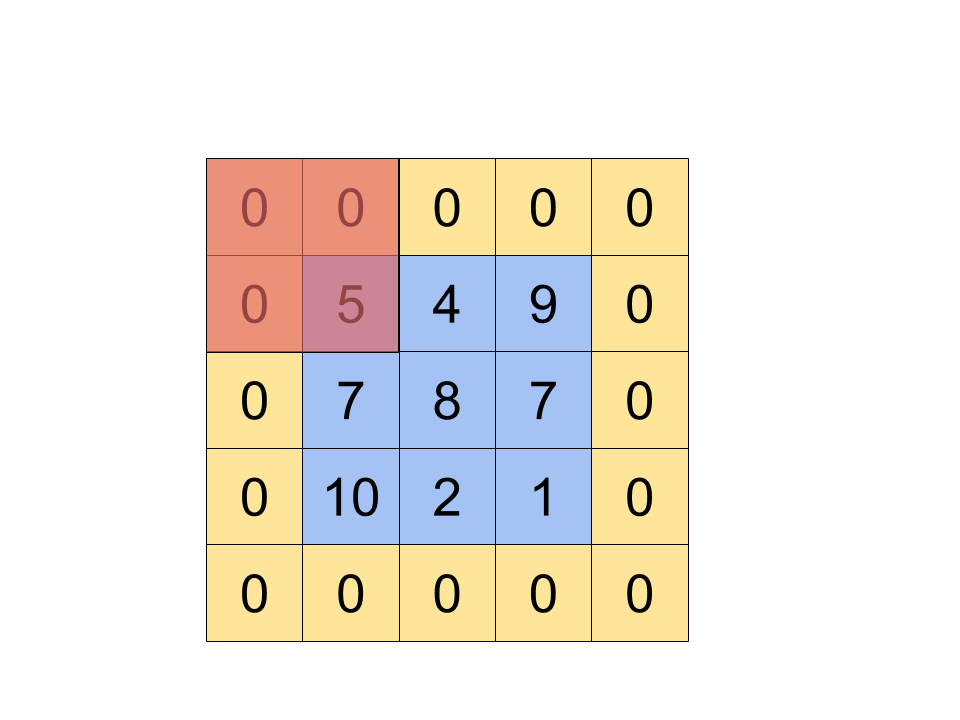
\includegraphics[width=.49\textwidth]{Plots/ConvolutionExample.png}
\end{center}
\begin{small}
Figure: A convolution being applied to a $2 \times 2$ patch (the red square) of a $3 \times 3$ image that has been zero-padded to allow convolutions past the edges of the image.
\end{small}

What is one benefit and one drawback to this zero-padding scheme (in contrast to an approach in which we only perform convolutions over patches entirely contained within an image)?

\begin{solution}

\end{solution}

\subsection{5 x 5 Convolutions}

Consider a single convolutional layer, where your input is a $32 \times 32$ pixel, RGB image. In other words, the input is a $32 \times 32 \times 3$ tensor. Your convolution has:

\begin{itemize}
\item Size: $5 \times 5 \times 3$
\item Filters: 8
\item Stride: 1
\item No zero-padding
\end{itemize}

\problem[2] What is the number of parameters (weights) in this layer, including a bias term? What is the shape of the output tensor?

\begin{subsolution}

\end{subsolution}


 \subsection{Max/Average Pooling}

Pooling is a downsampling technique for reducing the dimensionality of a layer's output. Pooling iterates across patches of an image similarly to a convolution, but pooling and convolutional layers compute their outputs differently: given a pooling layer $B$ with preceding layer $A$, the output of $B$ is some function (such as the max or average functions) applied to patches of $A$'s output.

Below is an example of max-pooling on a 2-D input space with a $2\times 2$ filter (the max function is applied to $2\times 2$ patches of the input) and a stride of 2 (so that the sampled patches do not overlap):

\begin{center}
  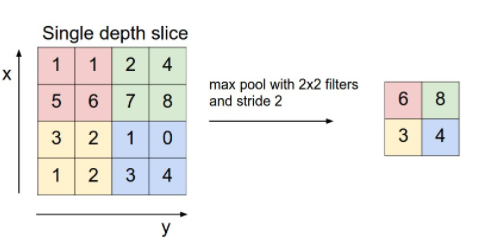
\includegraphics[width=.49\textwidth]{Plots/MaxPool.png}
\end{center}

Average pooling is similar except that you would take the average of each patch as its output instead of the maximum.

Consider the following 4 matrices:
$$
\begin{bmatrix}
    1 & 1 & 1 & 0 \\
    1 & 1 & 1 & 0 \\
    1 & 1 & 1 & 0 \\
    0 & 0 & 0 & 0
\end{bmatrix},
%
\begin{bmatrix}
    0 & 1 & 1 & 1 \\
    0 & 1 & 1 & 1 \\
    0 & 1 & 1 & 1 \\
    0 & 0 & 0 & 0
\end{bmatrix},
%
\begin{bmatrix}
	0 & 0 & 0 & 0 \\
    0 & 1 & 1 & 1 \\
    0 & 1 & 1 & 1 \\
    0 & 1 & 1 & 1
\end{bmatrix},
%
\begin{bmatrix}
    0 & 0 & 0 & 0 \\
    1 & 1 & 1 & 0 \\
    1 & 1 & 1 & 0 \\
    1 & 1 & 1 & 0
\end{bmatrix}
$$
\problem[3]

\begin{enumerate}
    \item Apply $2 \times 2$ average pooling with a stride of 2 to each of the above images.
    \item Apply $2 \times 2$ max pooling with a stride of 2 to each of the above images.
\end{enumerate}

\begin{subsolution}
\begin{enumerate}
    \item Average pooling:
    \item Max pooling:
\end{enumerate}
\end{subsolution}


\problem[4]

Consider a scenario in which we wish to classify a dataset of images of various animals, taken at various angles/locations and containing small amounts of noise (e.g. some pixels may be missing). Why might pooling be advantageous given these distortions in our dataset?

\begin{subsolution}

\end{subsolution}

\subsection{Hyperparameter Tuning}
The performance of neural networks depends to a large extent on the choice of hyperparameters. However, theory does not give us a systematic way of how to pick them. In practice, there are at least three different strategies to tune a network.

\begin{enumerate}
    \item \textbf{"Babysitting":} When tuning a model, you can manually choose a set of hyperparameters, monitor in- and out-of-sample performance, adjust according to intuition, and train again.

    \item \textbf{Grid search:} For each hyperparameter (learning rate, dropout probability, etc), you define a \textit{range} of values to search, and an \textit{interval} at which to sample points. For example, you could try learning rates lr$=\{10^{-1}, 10^{-2}, \ldots, 10^{-5}\}$ and dropout probabilities $p=\{0, 0.1, \ldots, 0.5\}$, and then train your model for each (lr, p) pair, and keep the setting that yields best results.

    \item \textbf{Random search:} You can again define a search range, but instead of testing points at pre-determined intervals, you could sample points at random and train your model with those hyperparameters. You could take it one step further and implement a "coarse-to-fine" approach: i.e. define a large search space, sample and test a few hyperparameters, and then repeat the process inside a finer search space around those hyperparameters that yielded best results in the first pass.
\end{enumerate}
\problem[5] Pick one of the three hyperparameter tuning strategies, and explain at least one strength and one limitation of using that strategy to tune your model.

\begin{subsolution}

\end{subsolution}

\subsection{PyTorch implementation}
\problem[20]

Using PyTorch ``Sequential'' model class as you did in 2C, build a deep \emph{convolutional}
network to classify the handwritten digits in MNIST. You are now allowed to use
the following layers (but \textbf{only} the following):

 \begin{itemize}
  \item \textbf{Linear:} A fully-connected layer
  \begin{itemize}
    \item In convolutional networks, Linear (also called dense) layers are typically used to knit together higher-level feature representations.
    \item Particularly useful to map the 2D features resulting from the last convolutional layer to categories for classification (like the 1000 categories of ImageNet or the 10 categories of MNIST).
    \item Inefficient use of parameters and often overkill: for $A$ input activations and $B$ output activations, number of parameters needed scales as $O(AB)$.
  \end{itemize}
  \item \textbf{Conv2d:} A 2-dimensional convolutional layer
  \begin{itemize}
    \item The bread and butter of convolutional networks, conv layers impose a translational-invariance prior on a fully-connected network. By sliding filters across the image to form another image, conv layers perform ``coarse-graining'' of the image.
    \item Networking several convolutional layers in succession helps the convolutional network knit together more abstract representations of the input. As you go higher in a convolutional network, activations represent pixels, then edges, colors, and finally objects.
    \item More efficient use of parameters. For $N$ filters of $K \times K$ size on an input of size $L \times L$, the number of parameters needed scales as $O(N K^2)$. When $N, K$ are small, this can often beat the $O(L^4)$ scaling of a Linear layer applied to the $L^2$ pixels in the image.

  \end{itemize}
  \item \textbf{MaxPool2d:} A 2-dimensional max-pooling layer
  \begin{itemize}
    \item Another way of performing ``coarse-graining'' of images, max-pool layers are another way of ignoring finer-grained details by only considering maximum activations over small patches of the input.
    \item Drastically reduces the input size. Useful for reducing the number of parameters in your model.
    \item Typically used immediately following a series of convolutional-activation layers.
  \end{itemize}
  \item \textbf{BatchNorm2d:} Performs batch normalization (Ioffe and Szegedy, 2014). Normalizes the activations of previous layer to standard normal (mean 0, standard deviation 1).
  \begin{itemize}
    \item Accelerates convergence and improves performance of model, especially when saturating nonlinearities (sigmoid) are used.
    \item Makes model less sensitive to higher learning rates and initialization, and also acts as a form of regularization.
    \item Typically used immediately before nonlinearity (Activation) layers.
  \end{itemize}
  \item \textbf{Dropout:} Takes some probability and at every iteration sets weights to zero at random with that probability
  \begin{itemize}
    \item An effective form of regularization. During training, randomly selecting activations to shut off forces network to build in redundancies in the feature representation, so it does not rely on any single activation to perform classification.
  \end{itemize}
  \item \textbf{ReLU (activation):} Sets negative inputs to 0
  \item \textbf{Softmax (activation):} Rescales input so that it can be interpreted as a (discrete) probability distribution.
  \item \textbf{Flatten:} Flattens any tensor into a single vector (required in order to pass a 2D tensor output from a convolutional layer as input into Linear layers)
\end{itemize}

\textbf{Your tasks.} Build a network with only the allowed layers that achieves \textbf{test accuracy of at least 0.985}. You are required to use categorical cross entropy as your loss function and to train for 10 epochs with a batch size of 32. Note: your model must have fewer than 1 million parameters, as measured by the method given in the sample code.
Everything else can change: optimizer (RMSProp, Adam, ???), initial learning rates, dropout probabilities, layerwise regularizer strengths, etc. You are not required to use all of the layers, but \emph{you must have
at least one dropout layer and one batch normalization layer in your final model}. Try to figure out the best possible architecture and hyperparameters given these building blocks!

In order to design your model, you should train your model for 1 epoch (batch size 32) and look at the final \textbf{test accuracy}  after training. This should take no more than 10 minutes, and should give you an immediate sense for how fast your network converges and how good it is.

Set the probabilities of your
dropout layers to 10 equally-spaced values $p \in [0, 1]$, train for 1 epoch, and report the final model accuracies for each.

You can perform all of your hyperparameter validation in this way: vary your parameters and train for an epoch. After you're satisfied with the model design, you should train your model for the full 10 epochs.

\textbf{In your submission.} Turn in the code of your model, the test accuracy for the 10 dropout probabilities $p \in [0, 1]$, and the
final test accuracy when your model
is trained for 10 epochs. We should have everything needed to reproduce your results.

Discuss what you found to be the most effective strategies in designing a convolutional network. Which regularization method was most effective (dropout, layerwise regularization, batch norm)?

Do you foresee any problem with this way of validating our hyperparameters? If so, why?

\emph{Hints:}

\begin{itemize}
	\item You are provided with a sample network that achieves a high accuracy. Starting with this network, modify some of the regularization parameters (layerwise regularization strength, dropout probabilities) to see if you can maximize the test accuracy. You can also add layers or modify layers (e.g.
	changing the convolutional kernel sizes, number of filters, stride, dilation, etc.) so long as the total number of parameters remains under the cap of 1 million.
  \item You may want to read up on successful convolutional architectures, and emulate some of their design principles. Please cite any idea you use that is not your own.
  \item To better understand the function of each layer, check the PyTorch documentation.
  \item Linear layers take in single vector inputs (ex: \emph{(784, )}) but Conv2D layers
	take in tensor inputs (ex: \emph{(28, 28, 1)}): width, height, and channels. Using the transformation \verb$transforms.ToTensor()$ when loading the dataset will reshape the training/test $X$ to a 4-dimensional tensor (ex: \emph{(num_examples, width, height, channels)}) and normalize values. For the MNIST dataset, \emph{channels=1}. Typical color images have 3 color channels, 1 for each color in RGB.
	\item If your model is running slowly on your CPU, try making each layer smaller
	and stacking more layers so you can leverage deeper representations.
	\item Other useful CNN design principles:
  \begin{itemize}
    \item CNNs perform well with many stacked convolutional layers, which develop increasingly large-scale representations of the input image.
    \item Dropout ensures that the learned representations are robust to some amount of noise.
    \item Batch norm is done after a convolutional or dense layer and immediately prior to an activation/nonlinearity layer.
    \item Max-pooling is typically done after a series of convolutions, in order to gradually reduce the size of the representation.
    \item Finally, the learned representation is passed into a dense layer (or two), and then filtered down to the final softmax layer.
  \end{itemize}
\end{itemize}
\begin{solution}

\end{solution}

\end{document}